\begin{frame}
	\frametitle{Estrutura da Estratégia Proposta}
		\only<1>{
			\framesubtitle{Diagrama}
			\begin{textblock*}{\linewidth}(0.3cm,2cm)
				\begin{figure}[h]
	\centering
	\caption{Estrutura da estratégia proposta}
	\scalebox{0.75}	{
		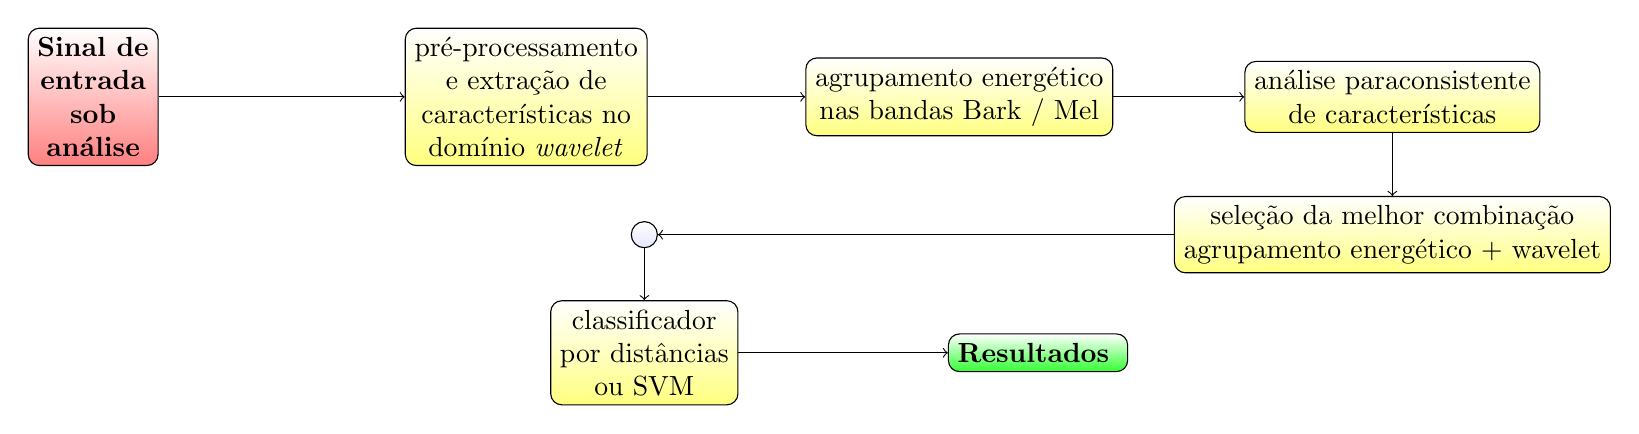
\begin{tikzpicture} 
			\node (z1)[shape=rectangle, rounded corners, draw, align=center, top color=white, bottom color=red!50] 
			at (0,2){
				\textbf{Sinal de} \\ \textbf{entrada} \\ \textbf{sob} \\ \textbf{análise}
			}; 
				
			\node (z2)[shape=rectangle, rounded corners, draw, align=center, top color=white, bottom color=yellow!50] 
			at (5.5,2){
				pré-processamento \\ e extração de \\ características no \\ domínio \textit{wavelet}
			}; 	
			
			\node (z3)[shape=rectangle, rounded corners, draw, align=center, top color=white, bottom color=yellow!50] 
			at (11,2){
				agrupamento energético \\ nas bandas Bark / Mel
			}; 	
			
			\node (z4)[shape=rectangle, rounded corners, draw, align=center, top color=white, bottom color=yellow!50] 
			at (16.5,2){
				análise paraconsistente \\ de características
			}; 
			
			\node (z5)[shape=rectangle, rounded corners, draw, align=center, top color=white, bottom color=yellow!50] 
			at (16.5,0.25){
				seleção da melhor combinação \\ agrupamento energético + wavelet
			}; 
					
			\node (z6)[shape=circle, draw, align=center, top color=white, bottom color=blue!10] 
			at (7,0.25) {};
			
			\node (z7)[shape=rectangle, rounded corners, draw, align=center, top color=white, bottom color=yellow!50] 
			at (7,-1.25) {
				classificador \\ por distâncias \\ ou SVM
			};
			
			\node (z8)[shape=rectangle, rounded corners, draw, align=center, top color=white, bottom color=green!80] 
			at (12,-1.25) {
				\textbf{Resultados}
			};
			
			\path[->] (z1) edge (z2);
			\path[->] (z2) edge (z3);
			\path[->] (z3) edge (z4);
			\path[->] (z4) edge (z5);
			\path[->] (z5) edge (z6);
			\path[->] (z6) edge (z7);	
			\path[->] (z7) edge (z8);
		\end{tikzpicture}
	}
	\label{fig_arq}
	\\Fonte: Elaborado pelo autor, 2021.
\end{figure}
			\end{textblock*}
		}
		\only<2>{
			\framesubtitle{Wavelets usadas}
				\begin{itemize}
					\item Haar.
					\item Beylkin com suporte 18.
					\item Vaidyanathan de suporte 24.
					\item Daubechies de	suportes 4 até 76.
					\item Symmlets com suportes 8, 16 e 32.
					\item Coiflets com suportes 6, 12, 18, 24 e 30.
				\end{itemize}
		}
		\only<3>{
			\framesubtitle{Métricas}
				\begin{itemize}
					\item Tabela de confusão.
					\begin{itemize}
						\item EER (Equal Error Rate).
						\item Acurácia e seu respectivo desvio padrão.
					\end{itemize}
				\end{itemize}
		}
		\only<4>{
			\framesubtitle{Tabela de confusão}
				\begin{itemize}
					\item \textbf{TP}: Quantidade de itens verdadeiros classificados como tal (\textit{True Positive}).
					\item \textbf{TN}: Quantidade de itens falsos classificados como tal (\textit{True Negative}).
					\item \textbf{FN}: Quantidade de itens verdadeiros classificados como falsos (\textit{False Negative}).
					\item \textbf{FP}: Quantidade de itens falsos classificados como verdadeiros (\textit{False Positive}).
				\end{itemize} 
				\begin{table}
\newcommand{\mc}[3]{\multicolumn{#1}{#2}{#3}}
\definecolor{tcB}{rgb}{0.447059,0.74902,0.266667}
\definecolor{tcC}{rgb}{0,0,0}
\definecolor{tcD}{rgb}{0,0.4,0.701961}
\definecolor{tcA}{rgb}{0.65098,0.65098,0.65098}
\begin{center}
	\begin{tabular}{ccc}
		% use packages: color,colortbl
		\mc{1}{l}{} & \mc{1}{>{\columncolor{tcA}}c}{\textbf{Verdadeiro}} & \mc{1}{>{\columncolor{tcA}}c}{\textbf{Falso}}\\

		\mc{1}{>{\columncolor{tcA}}r}{\textbf{Verdadeiro}} & \mc{1}{>{\columncolor{tcB}}c}{\textcolor{tcC}{VV}} & \mc{1}{>{\columncolor{tcD}}c}{\textcolor{tcC}{FV}}\\

		\mc{1}{>{\columncolor{tcA}}r}{\textbf{Falso}} & \mc{1}{>{\columncolor{tcD}}c}{\textcolor{tcC}{FF}} & \mc{1}{>{\columncolor{tcB}}c}{\textcolor{tcC}{VF}}
	\end{tabular}
	\caption{Exemplo de matriz de confusão}
	\label{tab:confusionMatrixSample}
\end{center}
\end{table}

		}
		\only<5>{
			\framesubtitle{Acurácia e EER}
				\begin{columns}
					\column{.5\textwidth}
					\begin{equation}
						acuracia = \dfrac{TP + TN}{N} \qquad,
						\label{eq:calculoDaAcuracia}
					\end{equation}
					
					\column{.5\textwidth}
					\par São calculadas tabelas de confusão por um número suficiente de vezes até que \textbf{\textit{FAR} = \textit{FRR} = \textit{EER}}, a cada ciclo os vetores de características são comutados de forma aleatória.\newline

					\begin{equation}
						FAR=\dfrac{FP}{TN+FP} \qquad,
						\label{eq:FAR}
					\end{equation}
					
					\begin{equation}
						FRR=\dfrac{FN}{TP+FN} \qquad,
						\label{eq:FRR}
					\end{equation}
				\end{columns}
		}
\end{frame}